\documentclass[t]{beamer}
\usepackage{mathtools}
\usepackage{tikz}
\usepackage{pgfplots}
\usetikzlibrary{arrows,backgrounds,shapes,matrix,positioning,fit}
\newcommand{\argmax}{\operatornamewithlimits{argmax}}
\newcommand{\argmin}{\operatornamewithlimits{argmin}}
\newcommand{\wt}{\operatornamewithlimits{wt}}
\renewcommand\Re{\operatorname{Re}}
\renewcommand\Im{\operatorname{Im}}

\mode<presentation>
{
  \usetheme{Singapore}
  %\useoutertheme{infolines} % Showing only current section in navigation
  \setbeamertemplate{headline}{}  % Empty headline
  \setbeamertemplate{footline}[frame number]  % Getting rid of footer items except slide number
  \setbeamercovered{invisible}
  \beamertemplatenavigationsymbolsempty % Getting rid of navigation bullets at the bottom
}
\usepackage[english]{babel}
\usepackage[latin1]{inputenc}
\usepackage{times}
\usepackage[T1]{fontenc}

\title[EE 703 DMT]{Complex Baseband Representation}
\author[Saravanan V]
{
  Saravanan Vijayakumaran\\
  \href{mailto:sarva@ee.iitb.ac.in}{sarva@ee.iitb.ac.in}
}
\institute[IIT Bombay]
{
  Department of Electrical Engineering\\
  Indian Institute of Technology Bombay
}
\date{July 23, 2013}

\AtBeginSection[]%
{%
\begin{frame}[plain]%
  \topskip0pt
  \vspace*{\fill}
    \begin{center}%
      \usebeamerfont{section title}\insertsection%
    \end{center}%
  \vspace*{\fill}
\end{frame}%
}

\begin{document}

%% Frame %%
\begin{frame}
  \titlepage
\end{frame}

%% Frame %%
\begin{frame}{Baseband Signals}
  \begin{equation*}
    S(f) = 0, \ \ \ |f| > W  
  \end{equation*}
  \begin{figure}
    \centering
      \begin{tikzpicture}[scale=1.0,transform shape]
        \begin{axis}[
                     xlabel=$f$,
                     ylabel=$|S(f)|$,
                     xmax=2,
                     xmin=-2,
                     ymax=2,
                     ymin=-1,
                     %axis lines = middle,
                     axis x line = middle,
                     axis y line = middle,
                     ytick=\empty,
                     xtick = {-1,0,1},
                     xticklabels = {$-W$,$0$,$W$},
                    ]
          \addplot[color=blue,very thick] coordinates {(-1,0) (0,1) (1,0)};
          \addplot[color=red] coordinates {(-2,0) (2,0)};
        \end{axis}
\end{tikzpicture}
  \end{figure}
\end{frame}

%% Frame %%
\begin{frame}{Passband Signals}
  \begin{equation*}
    S(f) \neq 0, \ \ \ |f\pm f_c| \leq W, \ \ \  f_c > W > 0.
  \end{equation*}
  \begin{figure}
    \centering
      \begin{tikzpicture}[scale=1.0,transform shape]
        \begin{axis}[
                     xlabel=$f$,
                     ylabel=$|S_p(f)|$,
                     xmax=6,
                     xmin=-6,
                     ymax=2,
                     ymin=-1,
                     ytick=\empty,
                     axis lines = middle,
                     xtick = {-5,-3,-1,1,3,5},
                     xticklabels = {$-f_c-W$,$-f_c$,$-f_c+W$,$f_c-W$,$f_c$,$f_c+W$},
                     %x tick label style={font=\tiny}
                     x post scale = 1.5
                    ]
          \addplot[color=blue,very thick] coordinates {(-5,0) (-3,1) (-1,0) };
          \addplot[color=blue,very thick] coordinates { (1,0) (3,1) (5,0)};
        \end{axis}
      \end{tikzpicture}
  \end{figure}
\end{frame}

%% Frame %%
\begin{frame}{Sampling Theorem}
  \pause
  \begin{theorem}
  If a signal $s(t)$ is bandlimited to $B$, 
  \begin{equation*}
    S(f) = 0, \ \ \ |f| > B  
  \end{equation*}
  then a sufficient condition for exact reconstructability is a uniform sampling rate $f_s$ where
  \pause
  \begin{equation*}
  f_s > 2B.
  \end{equation*}
  \end{theorem}
  \pause
  \begin{description}
    \item[Baseband Signals] $B = \pause W$
    \pause
    \item[Passband Signals] $B = \pause f_c+W$ \pause \alert{(Can we do better?)}
  \end{description}
\end{frame}

%% Frame %%
\begin{frame}{Fourier Transform for Real Signals}
\begin{eqnarray*}
  \Im[s(t)] = 0  & \Rightarrow \pause & S(f) = S^*(-f) \ \ \ \ \ \ \ \text{(Conjugate Symmetry)} \\
                 \pause
                 & \Rightarrow  & |S(f)| = |S(-f)|, \  \arg(S(f)) = -\arg(S(-f))
\end{eqnarray*}
\pause
\begin{columns}
  \begin{column}{0.5\textwidth}
  \begin{figure}
    \centering
      \begin{tikzpicture}[scale=0.6,transform shape]
        \begin{axis}[
                     %xlabel=$f$,
                     title=$\Re(S(f))$,
                     xmax=2,
                     xmin=-2,
                     ymax=1.5,
                     ymin=-1.25,
                     axis lines = middle,
                     ytick={1,0},
                     xtick = {-1,0,1,2},
                     xticklabels = {$-W$,$0$,$W$,$f$},
                     yticklabels = {1,0},
                    ]
          \addplot[color=blue,very thick] coordinates {(-1,0) (0,1) (1,0)};
        \end{axis}
      \end{tikzpicture}
  \end{figure}
\end{column}

\begin{column}{0.5\textwidth}
  \begin{figure}
    \centering
      \begin{tikzpicture}[scale=0.6,transform shape]
        \begin{axis}[
                     %xlabel=$f$,
                     title=$\Im(S(f))$,
                     xmax=2,
                     xmin=-2,
                     ymax=1.5,
                     ymin=-1.25,
                     axis lines = middle,
                     ytick={1,-1},
                     xtick = {-1,0,1,2},
                     xticklabels = {$-W$,$0$,$W$,$f$},
                     yticklabels = {1,-1},
                    ]
          \addplot[color=blue,very thick] coordinates {(-1,0) (-1,1) (0,1) (0,-1) (1,-1) (1,0)};
        \end{axis}
      \end{tikzpicture}
  \end{figure}
  \end{column}
\end{columns}
\end{frame}

%% Frame %%
\begin{frame}{Fourier Transform of a Real Passband Signal}
  \begin{figure}
    \centering
      \begin{tikzpicture}[scale=0.4,transform shape]
        \begin{axis}[
                     title=$\Re(S_p(f))$,
                     xmax=7,
                     xmin=-7,
                     ymax=1.5,
                     ymin=-1.1,
                     axis lines = middle,
                     ytick=\empty,
                     xtick = {-5,5,7},
                     xticklabels = {$-f_c$,$f_c$,$f$},
                     %x tick label style={font=\tiny},
                     x post scale = 3.0
                    ]
          \addplot[color=blue,very thick] coordinates {(-6,0) (-4,1) (-4,0)};
          \addplot[color=blue,very thick] coordinates {(6,0) (4,1) (4,0)};
        \end{axis}
      \end{tikzpicture}
  \end{figure}

  \begin{figure}
    \centering
      \begin{tikzpicture}[scale=0.4,transform shape]
        \begin{axis}[
                     title=$\Im(S_p(f))$,
                     xmax=7,
                     xmin=-7,
                     ymax=1.5,
                     ymin=-1.1,
                     axis lines = middle,
                     ytick=\empty,
                     xtick = {-5,5,7},
                     xticklabels = {$-f_c$,$f_c$,$f$},
                     %x tick label style={font=\tiny},
                     x post scale = 3.0
                    ]
          \addplot[color=blue,very thick] coordinates {(-6,0) (-6,-1) (-4,-1) (-4,0)};
          \addplot[color=blue,very thick] coordinates {(6,0) (6,1) (4,1) (4,0)};
        \end{axis}
      \end{tikzpicture}
  \end{figure}
\end{frame}

%% Frame %%
\begin{frame}{Positive Spectrum of a Real Passband Signal}
  \begin{figure}
    \centering
      \begin{tikzpicture}[scale=0.4,transform shape]
        \begin{axis}[
                     title=$\Re(S_p^+(f))$,
                     xmax=7,
                     xmin=-7,
                     ymax=1.5,
                     ymin=-1.1,
                     axis lines = middle,
                     ytick=\empty,
                     xtick = {-5,5,7},
                     xticklabels = {$-f_c$,$f_c$,$f$},
                     %x tick label style={font=\tiny},
                     x post scale = 3.0
                    ]
          \addplot[color=blue,very thick] coordinates {(6,0) (4,1) (4,0)};
        \end{axis}
      \end{tikzpicture}
  \end{figure}

  \begin{figure}
    \centering
      \begin{tikzpicture}[scale=0.4,transform shape]
        \begin{axis}[
                     title=$\Im(S_p^+(f))$,
                     xmax=7,
                     xmin=-7,
                     ymax=1.5,
                     ymin=-1.1,
                     axis lines = middle,
                     ytick=\empty,
                     xtick = {-5,5,7},
                     xticklabels = {$-f_c$,$f_c$,$f$},
                     %x tick label style={font=\tiny},
                     x post scale = 3.0
                    ]
          \addplot[color=blue,very thick] coordinates {(6,0) (6,1) (4,1) (4,0)};
        \end{axis}
      \end{tikzpicture}
  \end{figure}
  \pause
  \begin{equation*}
     S_p^+(f) = S_p(f)u(f) 
  \end{equation*}
\end{frame}

%% Frame %%
\begin{frame}{Complex Envelope of a Real Passband Signal}
  \begin{figure}
    \centering
      \begin{tikzpicture}[scale=0.4,transform shape]
        \begin{axis}[
                     title=$\Re(S(f))$,
                     xmax=7,
                     xmin=-7,
                     ymax=1.5,
                     ymin=-1.1,
                     axis lines = middle,
                     ytick=\empty,
                     xtick = {7},
                     xticklabels = {$f$},
                     %x tick label style={font=\tiny},
                     x post scale = 3.0
                    ]
          \addplot[color=blue,very thick] coordinates {(1,0) (-1,1.414) (-1,0)};
        \end{axis}
      \end{tikzpicture}
  \end{figure}

  \begin{figure}
    \centering
      \begin{tikzpicture}[scale=0.4,transform shape]
        \begin{axis}[
                     title=$\Im(S(f))$,
                     xmax=7,
                     xmin=-7,
                     ymax=1.5,
                     ymin=-1.1,
                     axis lines = middle,
                     ytick=\empty,
                     xtick = {7},
                     xticklabels = {$f$},
                     %x tick label style={font=\tiny},
                     x post scale = 3.0
                    ]
          \addplot[color=blue,very thick] coordinates {(1,0) (1,1.414) (-1,1.414) (-1,0)};
        \end{axis}
      \end{tikzpicture}
  \end{figure}
  \pause
  \begin{equation*}
     S(f) = \sqrt{2} S_p^+(f+f_c) = \sqrt{2} S_p(f+f_c)u(f+f_c) 
  \end{equation*}
\end{frame}

%% Frame %%
\begin{frame}{Complex Envelope in Time Domain}
Frequency Domain Representation
  \begin{equation*}
     S(f) = \sqrt{2} S_p^+(f+f_c) = \sqrt{2} S_p(f+f_c)u(f+f_c) 
  \end{equation*}
  \pause
  Time Domain Representation of Positive Spectrum
  \begin{eqnarray*}
     S_p^+(f) & = & S_p(f)u(f) \\
     \pause
     s_p^+(t) & = & \pause s_p(t) \star \mathcal{F}^{-1}\left[u(f)\right]
  \end{eqnarray*}
  \pause
  Time Domain Representation of Frequency Domain Unit Step
  \begin{eqnarray*}
     u(t) & \xrightleftharpoons{} & \pause \frac{1}{j2\pi f} + \frac{1}{2}\delta(f) \\
     \pause
     u(f) & \xrightleftharpoons{} & \pause \frac{1}{-j2\pi t} + \frac{1}{2}\delta(-t) \\
     \pause
          &  & = \frac{j}{2\pi t} + \frac{1}{2}\delta(t) 
  \end{eqnarray*}
\end{frame}

%% Frame %%
\begin{frame}{Complex Envelope in Time Domain}
  Time Domain Representation of Positive Spectrum
  \begin{eqnarray*}
     s_p^+(t) & = & s_p(t) \star \left[ \frac{1}{2}\delta(t) + \frac{j}{2\pi t}  \right] \\
     \pause   
              & = & \frac{1}{2} \left[ s_p(t) + j\hat{s}_p(t) \right]
  \end{eqnarray*}
  \pause 
  Time Domain Representation of Complex Envelope
  \begin{eqnarray*}
    \sqrt{2}S_p(f)u(f) & \xrightleftharpoons{} & \frac{1}{\sqrt{2}} \left[ s_p(t) + j\hat{s}_p(t) \right] \\
    \pause
    \sqrt{2}S_p(f+f_c)u(f+f_c) & \xrightleftharpoons{} & \pause \frac{1}{\sqrt{2}} \left[ s_p(t) + j\hat{s}_p(t) \right] e^{-j2\pi f_ct} \\
    \pause
    S(f) & \xrightleftharpoons{} & \pause \frac{1}{\sqrt{2}} \left[ s_p(t) + j\hat{s}_p(t) \right] e^{-j2\pi f_ct} \\
    \pause
    s(t) & = & \frac{1}{\sqrt{2}} \left[ s_p(t) + j\hat{s}_p(t) \right] e^{-j2\pi f_ct} 
  \end{eqnarray*}
\end{frame}

%% Frame %%

\begin{frame}{Passband Signal in terms of Complex Envelope}
  Complex Envelope
  \begin{equation*}
  s(t) = s_c(t) + js_s(t)
  \end{equation*}
    \begin{description}
      \item[$s_c(t)$] In-phase component
      \item[$s_s(t)$] Quadrature component
    \end{description}
  \pause
  Time Domain Relationship
  \begin{eqnarray*}
  s_p(t) & = & \pause \Re\left[\sqrt{2}s(t)e^{j2\pi f_c t}\right] \\
         \pause
         & = & \Re\left[\sqrt{2}\{s_c(t)+js_s(t)\}e^{j2\pi f_c t}\right] \\
         \pause
         & = & \sqrt{2}s_c(t)\cos 2\pi f_ct - \sqrt{2}s_s(t)\sin 2\pi f_c t
  \end{eqnarray*}
  \pause
  Frequency Domain Relationship
  \begin{equation*}
    S_p(f) = \pause \frac{S(f-f_c)+S^*(-f-f_c)}{\sqrt{2}}
  \end{equation*}
\end{frame}

%% Frame %%

\begin{frame}{Upconversion}
  \begin{equation*}
    s_p(t) = \sqrt{2}s_c(t)\cos 2\pi f_ct - \sqrt{2}s_s(t)\sin 2\pi f_c t
  \end{equation*}
  \pause
  \begin{figure}
    \centering
      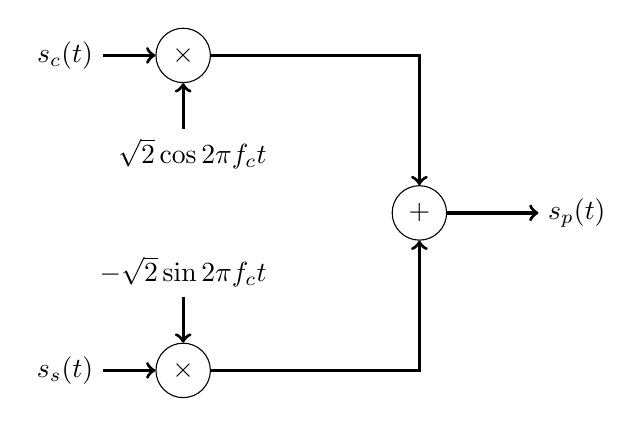
\begin{tikzpicture}[scale=1.0,transform shape]
      \node at (-0.5,2) (sc) {$s_c(t)$};
      \node at (-0.5,-2) (ss) {$s_s(t)$};
      \node[circle, draw, minimum size = 5mm] at (1,2) (prodc) {$\times$};
      \node[circle, draw, minimum size = 5mm] at (1,-2) (prods) {$\times$};
      \node[circle, draw, minimum size = 5mm] at (4,0) (adder) {$+$};
      \node at (1,0.75) (cos) {$\ \ \sqrt{2}\cos 2\pi f_ct$};
      \node at (1,-0.75) (sin) {$-\sqrt{2}\sin 2\pi f_ct$};
      \node at (6,0) (sp) {$s_p(t)$};
      \draw[->,very thick] (sc) -- (prodc);
      \draw[->,very thick] (ss) -- (prods);
      \draw[->,very thick] (prodc) -| (adder);
      \draw[->,very thick] (prods) -| (adder);
      \draw[->,very thick] (cos) -- (prodc);
      \draw[->,very thick] (sin) -- (prods);
      \draw[->,very thick] (adder) -- (sp);
      \end{tikzpicture}
  \end{figure}
\end{frame}

%% Frame %%
\begin{frame}{Downconversion}
  \pause
  \begin{eqnarray*}
    \sqrt{2}s_p(t)\cos 2\pi f_ct & = & 2s_c(t)\cos^2 2\pi f_ct - 2 s_s(t)\sin 2\pi f_c t \cos 2\pi f_c t\\
    \pause
        & = & s_c(t) + s_c(t)\cos 4\pi f_ct-s_s(t)\sin 4\pi f_ct
  \end{eqnarray*}
  \pause
  \begin{figure}
    \centering
      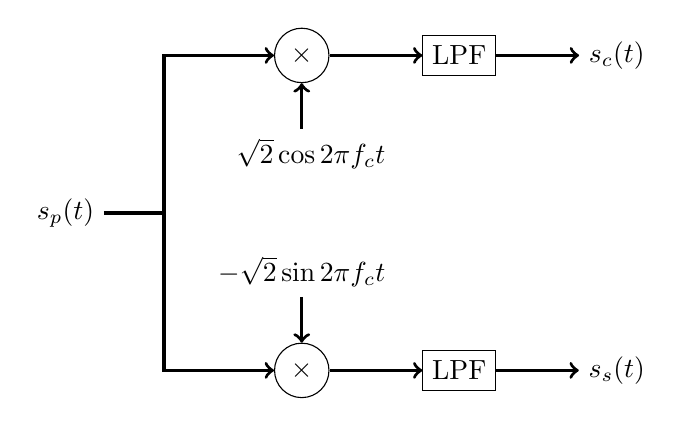
\begin{tikzpicture}[scale=1.0,transform shape]
      \node at (5,2) (sc) {$s_c(t)$};
      \node at (5,-2) (ss) {$s_s(t)$};
      \node[circle, draw, minimum size = 5mm] at (1,2) (prodc) {$\times$};
      \node[circle, draw, minimum size = 5mm] at (1,-2) (prods) {$\times$};
      \node[rectangle, draw, minimum size = 5mm] at (3,2) (LPc) {LPF};
      \node[rectangle, draw, minimum size = 5mm] at (3,-2) (LPs) {LPF};
      \node at (1,0.75) (cos) {$\ \ \sqrt{2}\cos 2\pi f_ct$};
      \node at (1,-0.75) (sin) {$-\sqrt{2}\sin 2\pi f_ct$};
      \node at (-2,0) (sp) {$s_p(t)$};
      \draw[->,very thick] (prodc) -- (LPc);
      \draw[->,very thick] (prods) -- (LPs);
      \draw[->,very thick] (LPc) -- (sc);
      \draw[->,very thick] (LPs) -- (ss);
      \draw[->,very thick] (cos) -- (prodc);
      \draw[->,very thick] (sin) -- (prods);
      \draw[->,very thick] (-0.75,0) |- (prodc);
      \draw[->,very thick] (-0.75,0) |- (prods);
      \draw[very thick] (sp) -- (-0.75,0);
      \end{tikzpicture}
  \end{figure}
\end{frame}

%% Frame %%
\begin{frame}{Inner Product and Energy}
  Let $s(t)$ and $r(t)$ be signals. 
  \pause
  \begin{definition}[Inner Product]
    \begin{equation*}
      \langle s,r \rangle = \int_{-\infty}^{\infty} s(t)r^*(t)\ dt
    \end{equation*}
  \end{definition}
  \pause
  \begin{definition}[Energy]
    \begin{equation*}
      E_s = \lVert s \rVert^2 = \langle s,s \rangle = \int_{-\infty}^{\infty} \lvert s(t)\rvert^2 \ dt
    \end{equation*}
  \end{definition}
\end{frame}

%% Frame %%
\begin{frame}{$I$ and $Q$ Channels of a Passband Signal}
  \begin{equation*}
    s_p(t) = \underbrace{\sqrt{2}s_c(t)\cos 2\pi f_ct}_{I \text{ Component}}- \underbrace{\sqrt{2}s_s(t)\sin 2\pi f_c t}_{Q \text{ Component}}
  \end{equation*}
  \pause
  \begin{eqnarray*}
    x_c(t) & = & \sqrt{2}s_c(t)\cos 2\pi f_ct \\
    x_s(t) & = & \sqrt{2}s_s(t)\sin 2\pi f_ct
  \end{eqnarray*}
  \pause
  \begin{center}
    $I$ and $Q$ Channels of a Passband Signal are Orthogonal
  \end{center}
  \begin{equation*}
    \langle x_c,x_s \rangle = 0
  \end{equation*}
\end{frame}

%% Frame %%
\begin{frame}{Passband and Baseband Inner Products}
  \begin{equation*}
    \langle u_p,v_p \rangle = \pause \langle u_c,v_c \rangle + \langle u_s,v_s \rangle = \pause \Re\left(\langle u,v \rangle\right)
  \end{equation*}
  \pause
  \begin{center}
    Energy of Complex Envelope = Energy of Passband Signal
  \end{center}
  \begin{equation*}
    \lVert s \rVert^2 = \lVert s_p \rVert^2
  \end{equation*}
\end{frame}

%% Frame %%
\begin{frame}{Complex Baseband Equivalent of Passband Filtering}
  \begin{description}
    \item[$s_p(t)$] Passband signal
    \item[$h_p(t)$] Impulse response of passband filter
    \item[$y_p(t)$] Filter output
  \end{description}
  \pause
  \begin{eqnarray*}
    y_p(t) & = & s_p(t) \star h_p(t) \\
    \pause
    Y_p(f) & = & S_p(f)H_p(f)
  \end{eqnarray*}
  \pause
  \begin{eqnarray*}
    S_+(f) & = & S_p(f)u(f) \\
    H_+(f) & = & H_p(f)u(f) \\
    Y_+(f) & = & Y_p(f)u(f) \\
    \pause
    Y_+(f) & = & S_+(f)H_+(f)
  \end{eqnarray*}
  \pause
  \begin{equation*}
    Y(f)  =  \sqrt{2}Y_+(f+f_c) = \sqrt{2}S_+(f+f_c)H_+(f+f_c) = \frac{1}{\sqrt{2}}S(f)H(f) 
  \end{equation*}
\end{frame}

%% Frame %%
\begin{frame}{Complex Baseband Equivalent of Passband Filtering}
\begin{eqnarray*}
y(t) & = & \frac{1}{\sqrt{2}} s(t) \star h(t)\\
\pause
y_c  & = &\frac{1}{\sqrt{2}}(s_c\star h_c - s_s \star h_s) \\
y_s  & = & \frac{1}{\sqrt{2}}(s_s\star h_c + s_c \star h_s) 
\end{eqnarray*}
\end{frame}
%% Frame %%
\begin{frame}{}
\vfill
\begin{center}
Thanks for your attention
\end{center}
\vfill
\end{frame}


\end{document}
